\documentclass[10pt]{beamer}

\usetheme[progressbar=frametitle]{metropolis}
\usepackage{mathtools}
\usepackage{booktabs}
\usepackage{setspace}
\usepackage{listings}

%\usepackage{pgfplots}
%\usepgfplotslibrary{dateplot}

\usepackage{xspace}
\newcommand{\order}[1]{\mathcal{O}(#1)}

%color definitions	
\definecolor{ourgreen}{rgb}{0,0.6,0}
\definecolor{ourgray}{rgb}{0.5,0.5,0.5}
\definecolor{ourmauve}{rgb}{0.58,0,0.82}

%code style
\lstset{ 
firstnumber=1,
language=python, % choose the language of the code
numbers=left,
stepnumber=1,% the step between two line-numbers. If it is 1 each line will be numbered
numbersep=5pt, % how far the line-numbers are from the code
frame=single,% adds a frame around the code
commentstyle=\color{ourgreen},    % comment style
keywordstyle=\color{blue},       % keyword style
stringstyle=\color{ourmauve},     % string literal style
breaklines=true, % sets automatic line breaking 
basicstyle=\tiny,
}



\title{Generating Trapdoor Primes}
\subtitle{A short take on generating SNFS primes}
% \date{\today}
\date{}
\author{Nikolai Rozanov}
\institute{UCL - Computer Science}
% \titlegraphic{\hfill\includegraphics[height=1.5cm]{logo.pdf}}

\begin{document}

\maketitle

%%%%%%%%%%%%%%%%%%%%%%%%%%%%%%%%%%%%%%%%%%%%%%%%%%%%%%
%
% TOC and Introduction
%
%%%%%%%%%%%%%%%%%%%%%%%%%%%%%%%%%%%%%%%%%%%%%%%%%%%%%%
\begin{frame}{Table of contents - Introduction}
  \setbeamertemplate{section in toc}[sections numbered]
  \tableofcontents[hideallsubsections]
\end{frame}



%%%%%%%%%%%%%%%%%%%%%%%%%%%%%%%%%%%%%%%%%%%%%%%%%%%%%%
%
% Importance
%
%%%%%%%%%%%%%%%%%%%%%%%%%%%%%%%%%%%%%%%%%%%%%%%%%%%%%%
\section{Importance}
\begin{frame}[fragile]{Importance}

\begin{itemize}
\item Look Up
\item Benchmarking
\item Deliberate Weakening
\end{itemize}



\end{frame}

%%%%%%%%%%%%%%%%%%%%%%%%%%%%%%%%%%%%%%%%%%%%%%%%%%%%%%
%
% Method and Code
%
%%%%%%%%%%%%%%%%%%%%%%%%%%%%%%%%%%%%%%%%%%%%%%%%%%%%%%
\section{Method and Code}

\begin{frame}[fragile]{Algorithm}
\begin{enumerate}[\textbf{Step} 1.]
\item Generating the prime q of the corresponding size.
\item Generating the coefficients for polynomials f and g, according to the size suggestions in \cite{Paper} 
\item Setting up a new polynomial G, which is the resultant of f and g and the variable is the leading coefficient of g.
\item Finding roots of G-1 modulo q, if there are no roots then going back to Step 1. 
\item Then letting p=$|G|$, and checking if p is prime, (an addition is to check whether q divides p-1).
\end{enumerate}
\end{frame}
\begin{frame}[fragile]{Main Script}
\textbf{Main Script}
\begin{lstlisting}
# Generating required Rings
X.<x>     = ZZ['x']
G.<x,g1>  = ZZ['x,g1']
# Main Loop
    #generating prime and Associated Field
    q = get_prime(bits_q)
    T.<g2>    = Integers(q)['g2']
	##while loop
        f_poly,norm_f = get_f(X,degree_f,bits_q)
        g_poly,g0 = get_g(g1,x,bits_p,degree_f, norm_f)
        G_poly = get_G(f_poly,g_poly)
        temp = list(G_poly.coefficients())
        temp.reverse()
        T2 = T(temp)
    r    = T2.roots()
    root = r[0][0]
    rt   = int(root)
#    while(rt<int(2^(bits_p/degree_f)/norm_f)):
#        rt+=q
    p    = X([G_poly(1,rt)+1])
\end{lstlisting}
\end{frame}




\begin{frame}[fragile]{Helper Functions}
\begin{alertblock}{Helper Functions}\end{alertblock}
\textbf{Prime Generation}
\begin{lstlisting}
def get_prime(bits_q):
    q = random_prime(2^bits_q-1,False,2^(bits_q-1))
    while(not is_prime(q)):
        q = random_prime(2^bits_q-1,False,2^(bits_q-1))
    return q
 \end{lstlisting}
 \textbf{Poly f}
 \begin{lstlisting}
def get_f(X,degree_f, bits_q):
    flag_irreducible = False
    while (not flag_irreducible):
        #f_vec = [ZZ.random_element(-int(2^(10)-1),int(2^(10)-1)) for _ in range(degree_f+1)]
        f_vec = [ZZ.random_element(-int(2^(bits_q/(2*(degree_f+1)))),int(2^(bits_q/(2*(degree_f+1))))) for _ in range(degree_f+1)]
        #f_vec = [ZZ.random_element(1,int(2^(bits_q/(2*(degree_f+1))))) for _ in range(degree_f+1)]

        norm_f = max(map(abs,f_vec))
        f_poly = X(list(f_vec))
        if f_poly.is_irreducible():
            flag_irreducible = True
    return f_poly,norm_f
        \end{lstlisting}
\end{frame}


\begin{frame}[fragile]{Helper Functions}
\textbf{Poly g}
 \begin{lstlisting}
def get_g(g1,x,bits_p,degree_f,norm_f):
    g0 = ZZ.random_element(-int(2^(bits_p/degree_f)/norm_f),int(2^(bits_p/degree_f)/norm_f))
    #g0 = ZZ.random_element(1,int(2^(bits_p/degree_f)/norm_f))
    g_poly = g1*x+g0
    return g_poly,g0
        \end{lstlisting}
\textbf{Poly G}
\begin{lstlisting}
def get_G(f_poly,g_poly):
    G_temp = f_poly.sylvester_matrix(g_poly,variable=x)
    G_poly = G_temp.determinant()-1
    return G_poly   
\end{lstlisting}
\end{frame}

%%%%%%%%%%%%%%%%%%%%%%%%%%%%%%%%%%%%%%%%%%%%%%%%%%%%%%
%
% Main Results
%
%%%%%%%%%%%%%%%%%%%%%%%%%%%%%%%%%%%%%%%%%%%%%%%%%%%%%%
\section{Some Analysis}

\begin{frame}[fragile]{Plots}
\textbf{Running Time Data}
\begin{figure}[H]
\minipage{0.9\textwidth}
  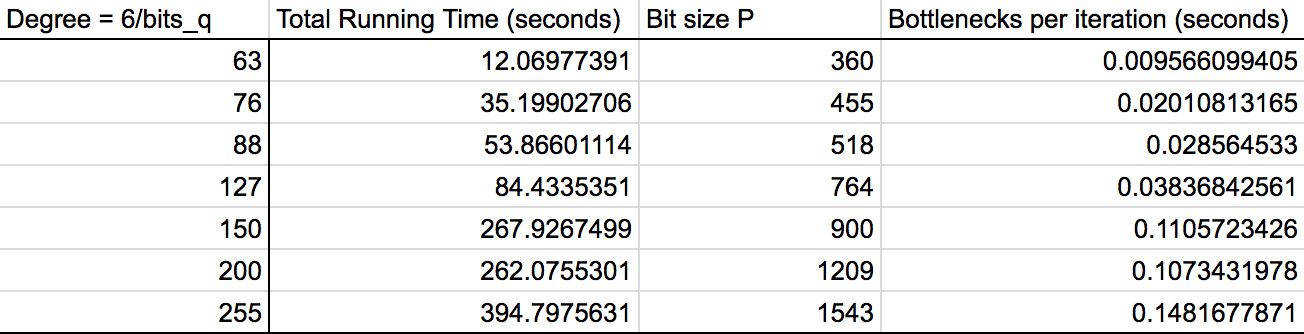
\includegraphics[width=\linewidth]{Data.png}
\endminipage
\end{figure}
\end{frame}


\begin{frame}[fragile]{Plots}
\textbf{Running Time Plot}
\begin{figure}[H]
\minipage{0.9\textwidth}
  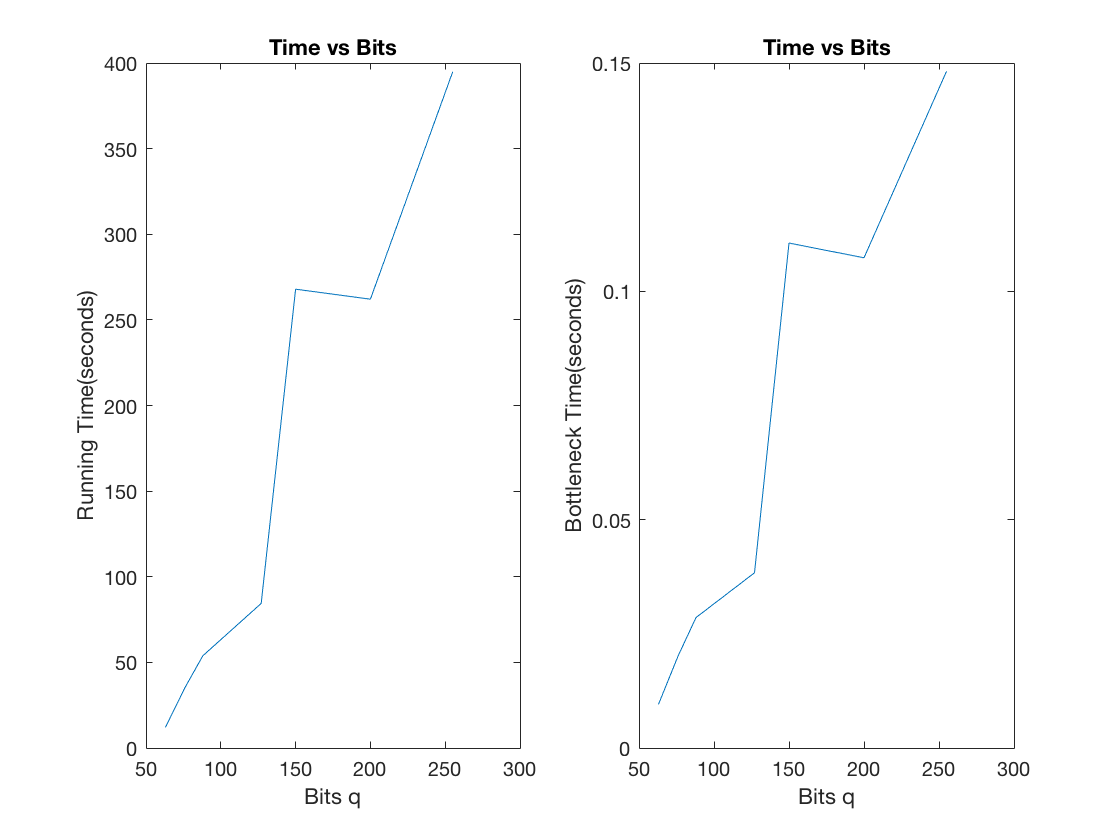
\includegraphics[width=\linewidth]{together.png}
\endminipage
\end{figure}
\end{frame}




\begin{frame}[allowframebreaks]{References}

  \bibliography{bibliography}
  \bibliographystyle{abbrv}

\end{frame}


\end{document}
